\documentclass[letterpaper,11pt]{article}
\usepackage{graphicx}
\usepackage{listings}

\lstset{
	basicstyle=\footnotesize,
	breaklines=true,
}

\begin{document}

\begin{titlepage}

\begin{center}

\Huge{Assignment 1}

\Large{CS 532:  Introduction to Web Science}

\Large{Spring 2016}

\Large{Manoj Chandra Kompalli}

\Large Finished on January 28,2016

\end{center}

\end{titlepage}

\newpage
\section*{1}

\subsection*{Question}

\begin{verbatim}
1.  Demonstrate that you know how to use "curl" well enough to
correctly POST data to a form.  Show that the HTML response that
is returned is "correct".  That is, the server should take the
arguments you POSTed and build a response accordingly.  Save the
HTML response to a file and then view that file in a browser and
take a screen shot.
\end{verbatim}


\subsection*{Answer}

I have started off with getting the response headers of the url’s. I then learnt to save the response header into a text file. I researched a bit and found out that the command to post data to a server. I quickly realized that due to security reasons most websites do not use the POST method. I could actually change the method to POST in my local machine if I wanted to.  Through the google groups page I found a url  https://www.cs.tut.fi/~jkorpela/forms/testing.html  . 
The response page shows the value of the input field from the requested page which was on http://www.cs.tut.fi/cgi-bin/run/~jkorpela/echo.cgi . Now, I used the curl command to POST the data on to the form using the command

\begin{lstlisting}[frame=single]
curl –-data “Content=hi_There_Manoj_here_!”  http://www.cs.tut.fi/cgi-bin/run/~jkorpela/echo.cgi
\end{lstlisting}

If we want to generate a file and save the response to it directly then,
\begin{lstlisting}[frame=single]
curl --data "Comment= hi_There_Manoj_here_!" http://www.cs.tut.fi/cgi-bin/run/~jkorpela/echo.cgi  -o p1.html
\end{lstlisting} 
where p1.html is the output page where the response is saved. 



\begin{figure}
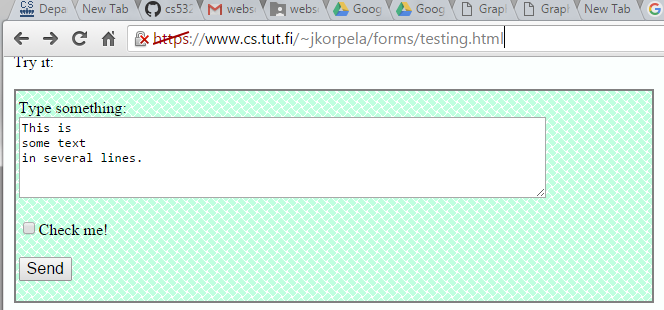
\includegraphics[scale=0.9]{requrl.png}
\caption{The form at https://www.cs.tut.fi/~jkorpela/forms/testing.html   where the request is made, rendered in Google Chrome}
\label{fig:screen1}
\end{figure}




\newpage



which renders in the browser like shown in Figure \ref{fig:q1screenie2}.

\begin{figure}
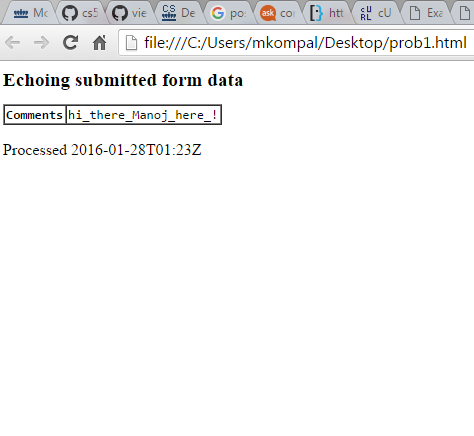
\includegraphics[scale=0.9]{response.png}
\caption{The response at http://www.cs.tut.fi/cgi-bin/run/~jkorpela/echo.cgi ,rendered in Google Chrome}
\label{fig:screen2}
\end{figure}

\begin{figure}
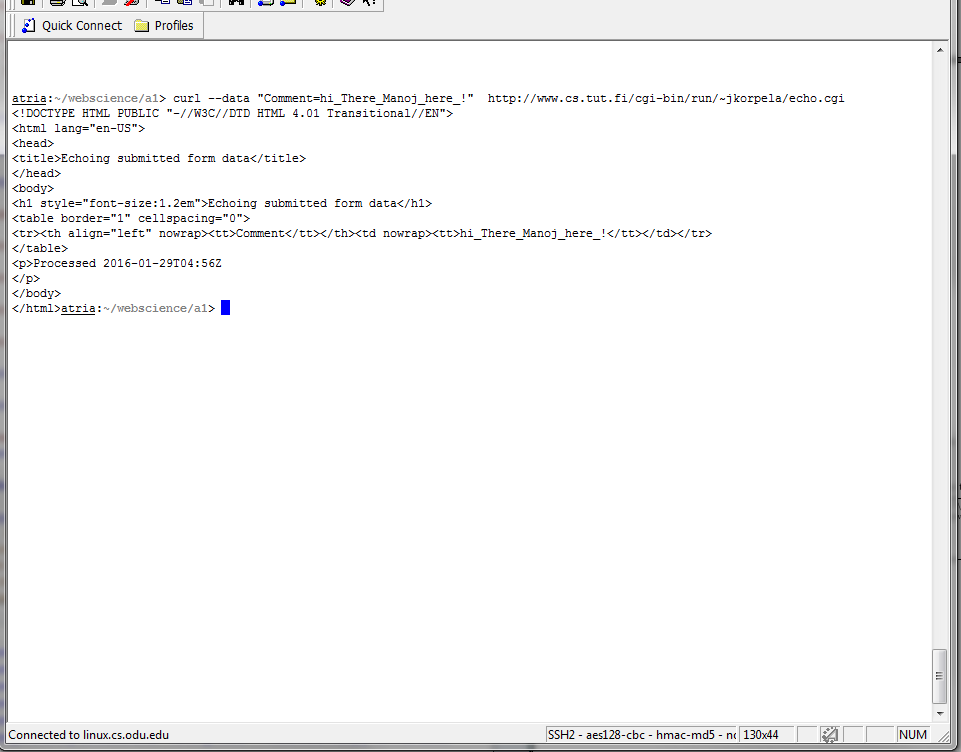
\includegraphics[scale=0.6]{shellresponse.png}
\caption{ Figure showing the response on secure shell CLI}
\label{fig:screen3}
\end{figure}




\newpage
\section*{2}

\subsection*{Question}





\begingroup
\fontsize{8pt}{10pt}\selectfont
\begin{verbatim}
2.  Write a Python program that:
  1. takes as a command line argument a web page
  2. extracts all the links from the page
  3. lists all the links that result in PDF files, and prints out
     the bytes for each of the links.  (note: be sure to follow
     all the redirects until the link terminates with a "200 OK".)
  4. show that the program works on 3 different URIs, one of which
     needs to be: 
     http://www.cs.odu.edu/~mln/teaching/cs532-s16/test/pdfs.html

3.  Consider the "bow-tie" graph in the Broder et al. paper (fig 9):
    http://www9.org/w9cdrom/160/160.html

\end{verbatim}
\endgroup


\newpage
\subsection*{Answer}
I have used the  BeautifulSoup library to extract all the links from a given url which is passed as a command line argument.I can use the findAll method which can extract specific html elements from the url.In my case I wanted to extract all the anchor tags. I also used urllib2 library which allows us to read the response header,parse the url and fetch the required content.I have used response.info() to get the response header elements like content type and content length. Now, I can list only the pdf urls by using filtering urls by content type. I found the size of the pdf in bytes using the response header attribute called content-length. Finally I displayed the status using response.getcode() .
Below is the python code which extracts urls which have pdf content and displays the size of pdf in bytes.
\subsection{Code Listing} 
\lstinputlisting[language=Python, breaklines=true]{prog2.py}
\begin{figure}
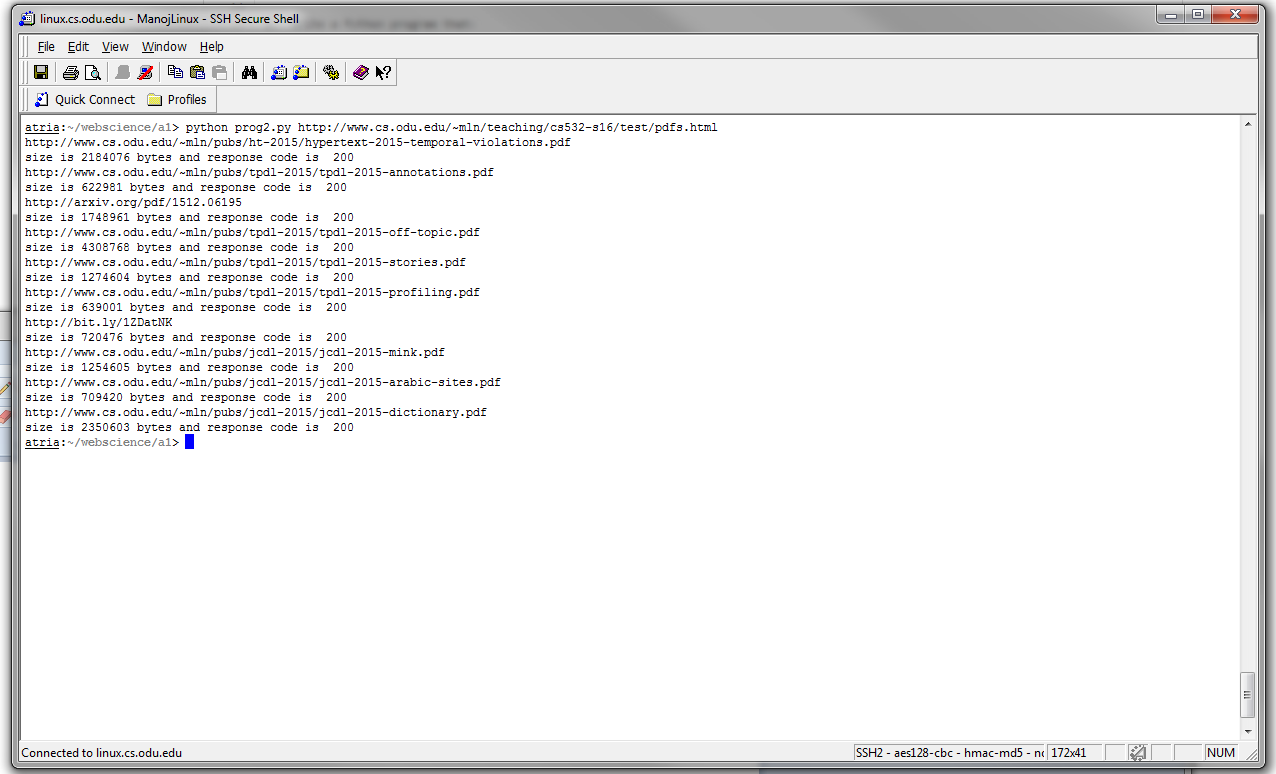
\includegraphics[scale=0.7]{nelsonurl.png}
\caption{ Figure showing the response for http://www9.org/w9cdrom/160/160.html}
\label{fig:screen4}
\end{figure}




\begin{figure}
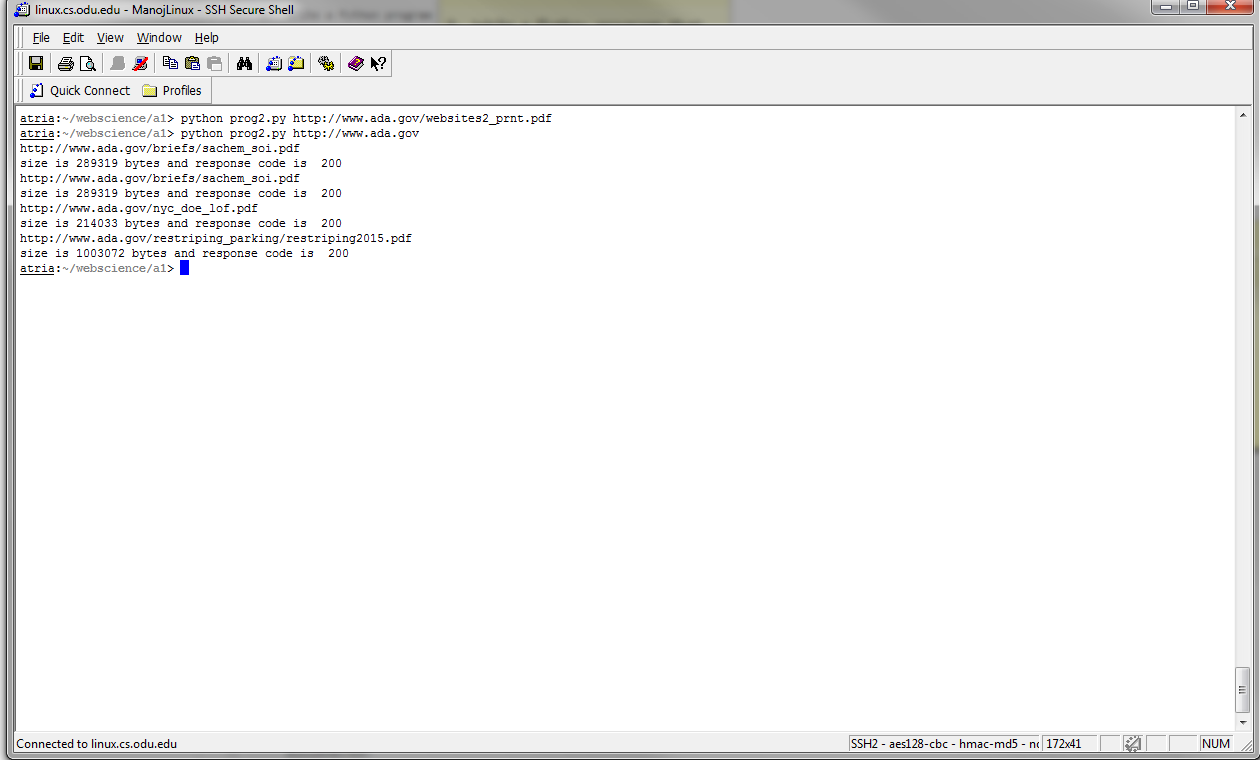
\includegraphics[scale=0.7]{adaurl.png}
\caption{ Figure showing the response for http://www.ada.gov}
\label{fig:screen6}
\end{figure}

\begin{figure}
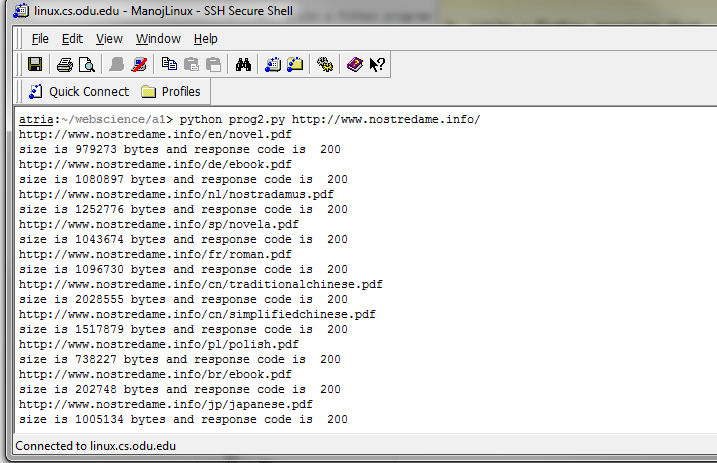
\includegraphics[scale=0.7]{novel.png}
\caption{ Figure showing the response for http://www.nostredame.info/}
\label{fig:screen7}
\end{figure}




\newpage




\newpage
\section*{3}

\subsection*{Question}

\begin{verbatim}
3.  Consider the "bow-tie" graph in the Broder et al. paper (fig 9):
    http://www9.org/w9cdrom/160/160.html

    Now consider the following graph:

    A --> B
    B --> C
    C --> D
    C --> A
    C --> G
    E --> F
    G --> C
    G --> H
    I --> H
    I --> J
    I --> K
    J --> D 
    L --> D
    M --> A
    M --> N
    N --> D
    O --> A
    P --> G 
    
    For the above graph, give the values for:

    IN: 
    SCC: 
    OUT: 
    Tendrils: 
    Tubes: 
    Disconnected:
\end{verbatim}

\newpage
\subsection*{Answer}
Figure \ref{fig:q3graph} is a graph of the included points, which looks like a bow-tie.

\begin{figure}
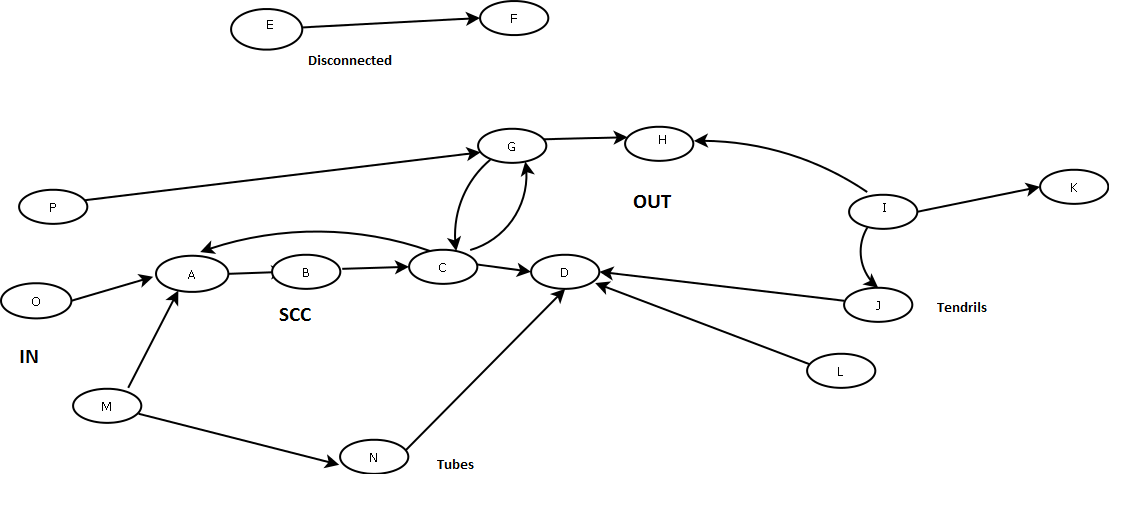
\includegraphics[scale=0.5]{graph.png}
\caption{Sketch of the above graph}
\label{fig:screen8}
\end{figure}

The descriptions of each node is a matter of interpretation.  Explanations have been provided for each value assignment.

\textbf{IN:}  $M, O, P$

IN is a set of nodes which are directed to the strongly connected nodes in the graph. In the graph we have $P, M,,O$ incident on $G,A,A$ respectively .$C$ is directed towards $A$ but it  is in SCC. Therefore $C$ is not a part of IN

\textbf{SCC:}  $A, B, C, G$

SCC is a set of strongly connected components which are linked to and from both IN and OUT. They are connected to every other node in SCC. $A,B,C,G$ fall under this category.

\textbf{OUT:}  $D,H$

OUT is a set of nodes which are directed from the nodes of SCC .Here we have $D,H$ in OUT

\textbf{Tendrils:}  $I, J, K, L$

The \emph{Tendrils} are pages that cannot reach the SCC or are not reached from the SCC.  The tendrils come from other graphs and only join the whole via $D,H$.

\textbf{Tubes:} $N$

\emph {Tubes} pass from IN to OUT without touching SCC. N is the tube which links from IN to OUT

\textbf{Disconnected:}  $E, F$

$E,F$ are the two nodes which are connected to each other but disconnected from the rest of the graph 
\newpage

\begin{thebibliography}{1}
\bibitem{one}
Curl tutorial, 
{\tt \\http://curl.haxx.se/docs/httpscripting.html }.

\bibitem{two}
Personal programming blog on python by Hemanth , 
{\tt  http://h3manth.com/content/methods-submit-form-post-using-curl-perl-python-ruby-lynx}.
\bibitem{three}
Python adventures wordpress blog , 
{\tt https://pythonadventures.wordpress.com/2011/03/10/extract-all-links-from-a-web-page/}.
\bibitem{four}
Python documentation , 
{\tt https://www.python.org/}.
\bibitem{five}
Broder et al. paper , 
{http://www9.org/w9cdrom/160/160.htm}.
\bibitem{six}
Dia tool for drawing charts.Installer , 
{http://dia-installer.de/download/index.html.en}.


\end{thebibliography}
 

\end{document}



